\clearpage
\setcounter{page}{1}
\maketitlesupplementary

\section{Training configuration}
\label{sec:suppl-config}

All methods share one nnU-Net~\cite{isensee2021nnunet} configuration; only
the input augmentation differs. Nothing below is tuned per dataset.

\paragraph{Training schedule.} 3D full-resolution nnU-Net, SGD with Nesterov
momentum $0.99$, initial learning rate $10^{-2}$ with the nnU-Net
\texttt{polyLR} decay, $250$ mini-batches per epoch, combined Dice and
cross-entropy loss, deep supervision on. Patch size, spacing and batch size
are whatever the nnU-Net planner selects for that dataset, identically for
every method. The epoch budget is fixed per dataset and shared by all methods
on it: $2500$ (Brats-GLI), $2000$ (ON-Harmony), $2000$ (Open-MS), $200$
(CHAOS). Every number reported in this paper is a 3-fold cross-validated
average; folds are the same across methods.

\paragraph{PALETTE hyper-parameters.} Set once and never tuned per dataset:
$k$-means class count drawn per sample from $\{2,\dots,6\}$, skipped in
favour of a single global remap with probability $0.10$; Voronoi
sub-parcellation of each intensity class with probability $0.60$ (else left
as one region); signed affine coefficient $\alpha \in \pm U(0.5, 2.0)$
applied per sub-region as in \cref{eq:affine} (always applied, to whatever
partition results from the $k$-means/Voronoi steps); per-label affine
decoupling applied independently per label with probability $0.5$ (skipped
for any label with under $4$ foreground voxels in that sample); Gaussian
blur $\sigma$ drawn from $\{0,0,0,0.3,0.5,0.8\}$, applied twice (after the
region-level and after the label-level remap), so mostly not applied at
either point. The transform is applied on the GPU, on-the-fly, to a fixed
$50\%$ of training
iterations (\emph{train050}); the remaining half of iterations use the
un-transformed real image.

\paragraph{Validation-time configuration.} \emph{val000} (the configuration
reported in the main paper) applies no synthetic contrast to the validation
split, matching every competing method and keeping model selection
like-for-like. \emph{val100} applies PALETTE to the entire validation split;
it is reported in \cref{sec:suppl-val100}.

\paragraph{Baseline configurations.} SynthSeg-noEM uses the authors' released
generator with its default priors. SynthSeg-EM is our re-implementation of
the variant described but not released in the original work; it estimates a
per-class intensity model from the sparse task labels available in each
dataset via expectation-maximization, and is otherwise identical in its
sampling procedure. SRCSM and Auglab use their published default
configurations. No competing method was re-tuned in our favour, and all use
the same folds, schedule and epoch budget as above.

\paragraph{Compute.} Training was performed on NVIDIA L40S and H100 GPUs. A
single fold costs from under an hour (CHAOS, $200$ epochs) to roughly three
days (Brats-GLI, $2500$ epochs); the full study is dominated by the $7$
methods $\times$ $8$ settings $\times$ $3$ folds main comparison plus the
ablation ladders of \cref{subsec:e-ablation}.


\section{Datasets and evaluation protocol}
\label{sec:suppl-data}

All evaluation is performed on held-out test cases only. For each task the model
is trained on a single source contrast and evaluated on every contrast of that
task's test split, including the training contrast itself; training and
validation subjects never appear in any reported number.

\paragraph{ON-Harmony} \cite{warrington2025onharmony} --- 31-region healthy-brain
segmentation. Reference labels are \emph{silver standard}: they were produced
automatically with FreeSurfer~\cite{fischl2012freesurfer} on the T1w volume of
each subject and then registered to that subject's other contrasts, which are
acquired in the same session. They are therefore not manual annotations, and
absolute Dice on this task should be read as agreement with an automated
reference rather than with a human rater; the comparison between methods, which
all use the identical reference, is unaffected.

\paragraph{Open-MS} \cite{lesjak2018openms} --- MS-lesion segmentation with
manual consensus annotations, evaluated across FLAIR, T1w and T2w.

\paragraph{Brats2024-GLI} \cite{deverdier2024brats2024} --- post-treatment
glioma sub-region segmentation, evaluated across T1n, T1c, T2w and T2-FLAIR.

\paragraph{CHAOS} \cite{kavur2021chaos} --- abdominal organ segmentation (liver,
spleen, both kidneys), evaluated across the CHAOS MR contrasts and, as a
cross-modality transfer, on held-out CT from AMOS~\cite{ji2022amos} and
SLIVER07~\cite{heimann2009comparison}.

\paragraph{ToothFairy2} \cite{bolelli2025toothfairy2} --- mandible segmentation
in dental cone-beam CT, the one non-CT, non-MRI training modality here. The
released label set is 42 classes, but annotation coverage is cohort-dependent:
several structures are annotated in only part of the cohort, so scoring them
would measure which cohort a case came from as much as the model. We therefore
reduce to the mandibular structures annotated throughout, and every column of
this task --- in-domain and cross-dataset alike --- is scored on that same
common label, so the numbers being averaged are commensurable. ToothFairy2
acquires CBCT only, so its held-out evidence is entirely
cross-modality: HaN-Seg~\cite{podobnik2023hanseg} head-and-neck CT and MR-T1.
Only HaN-Seg's CT arm is usable as a paired test; its MR is not registered to
its CT, and the MR-T1 column is scored against its own MR annotation.

\paragraph{I-SPY2 and Duke-Breast-MRI} \cite{li2022ispy2,saha2018duke} ---
breast-lesion segmentation. I-SPY2 (CC BY 4.0) is a neoadjuvant-chemotherapy
trial whose enrolment requires biopsy-proven invasive cancer, and its reference
is the trial's own functional tumour volume mask; training uses its
first-post-contrast T1 (T1-CE) and its T2w. Duke-Breast-MRI, obtained through
the MAMA-MIA release~\cite{garrucho2025mamamia} (CC BY-NC 4.0, so it carries a
non-commercial term the other cohorts here do not), is an external
cross-dataset test cohort only, contributing a T1-CE and a pre-contrast column.
Both are malignant-only cohorts with expert tumour masks. I-SPY2's DCE series
are acquired unilaterally at some sites and bilaterally at others; both
field-of-view variants are generated per patient rather than discarding either,
which is why the two training contrasts yield different test-case counts (102
for T1-CE, 168 for T2w) from the same 84 held-out patients.

\begin{table}[h]
\centering
\small
\setlength{\tabcolsep}{4pt}
\begin{tabular}{lcc}
\toprule
Task & Train & Test \\
\midrule
CHAOS          & 16  & 24 \\
ON-Harmony     & 84  & 8  \\
Open-MS        & 22  & 8  \\
Brats2024-GLI  & 630 & 70 \\
ToothFairy2    & 408 & 71 \\
I-SPY2         & 476 & 84 \\
\bottomrule
\end{tabular}
\caption{Per-task subject/case counts, pooled across the 3 folds used
everywhere in this paper ($\pm 1$ between folds). ON-Harmony counts are scan
sessions, not unique subjects, since its travelling-heads design scans some
subjects at multiple sites. CHAOS test includes its own held-out CT split,
separate from the AMOS/SLIVER07 cross-dataset transfer counted
independently (external cohorts, not re-tabulated here); likewise
ToothFairy2's HaN-Seg transfer and I-SPY2's Duke-Breast-MRI transfer. I-SPY2
counts are patients: each held-out patient yields one T1-CE case and, where
both field-of-view variants exist, more than one T2w case, giving the 102 and
168 per-contrast case counts quoted above. ToothFairy2 excludes one case with
no mandible label.}
\label{tab:suppl-datasets}
\end{table}


\section{Per-setting results}
\label{sec:suppl-persetting}

\cref{tab:meta} in the main paper reports results at the task level, pooling
each task's held-out test contrasts and both of its source modalities. This
section reports the same evaluation broken out into the eleven individual
source-modality settings. Every number is a cross-fold, cross-class average
over all held-out contrasts of that setting, under the protocol of
\cref{subsec:e-setup}.

\paragraph{Statistical test construction.} All tests are paired at the
level of the individual test case, never per-fold, so significance reflects
consistency across cases rather than aggregate noise. A case's score is its
mean over labels and over the evaluated folds, giving one observation per
held-out case; treating each fold's re-scoring of the same patient as an
independent sample would be pseudo-replication and would inflate the
effective sample size. Per-setting comparisons (below) use the paired
Wilcoxon signed-rank test~\cite{wilcoxon1945}, since there each setting is
judged on its own. All tests are Holm-corrected~\cite{holm1979} for multiple
comparisons.

\paragraph{Why the aggregate tests are sign-flip tests on a macro-average.}
The aggregate tests (\cref{tab:meta} and the per-dataset headline blocks)
are not paired Wilcoxon signed-rank tests, which is the more usual choice in
this literature: SynthSeg+, from the lineage we compare against, marks a
method as better than its competitors using a one-sided Bonferroni-corrected
Wilcoxon signed-rank test on paired Dice~\cite{billot2023synthsegplus}. We
therefore give our reason rather than leave it implicit. The \emph{estimand}
we test, by contrast, is not unusual at all --- it is the same
equal-weight-per-stratum principle the Medical Segmentation Decathlon
adopted, for the same reason, as set out below.

\emph{The estimand.} What we claim is $\text{macro}\Delta$: the mean, over
held-out contrasts, of that contrast's mean paired per-case difference
(ours minus competitor) --- equal weight per contrast, which is exactly what
the \emph{all} column of every table reports, so the test and the table
measure the same thing. Equal weighting is not cosmetic here. The claim
under test is cross-contrast generalization, and a contrast's held-out case
count reflects how large a public cohort happens to be, not how much that
contrast should say about generalizing. CHAOS is the extreme case: its
held-out CT evidence includes an external cohort contributing $200$ cases,
while each of its three MR contrasts contributes $8$. Weighting by case
count would let one CT cohort cast more than half the votes in a test whose
conclusion is about transfer across MR contrasts.

This is the same problem, and the same answer, as the Medical Segmentation
Decathlon's. Facing sample sizes that ``varied heavily across all tasks and
target ROIs,'' it ranked algorithms within each target ROI, averaged those
ranks per task, and averaged the per-task ranks for the final score ---
choosing that over a flat average across ROIs precisely because the flat
scheme means ``tasks with multiple target ROIs \ldots{} would be
over-weighted''~\cite{antonelli2022decathlon}. Our $\text{macro}\Delta$
applies the same principle one level across, with the held-out contrast in
place of the target ROI. Where we differ is only in how that weighted
quantity is reached: the Decathlon arrives at it through counts of pairwise
Wilcoxon outcomes at an uncorrected per-comparison $\alpha$, whereas we test
the weighted difference itself and Holm-correct across competitors.

\emph{Why not a pooled Wilcoxon.} The signed-rank test is defined on a
single undifferentiated sample of paired differences. Applying it to the
concatenation of all contrasts therefore tests a case-weighted null --- the
imbalance above, reintroduced --- and there is no standard reweighting of
the signed-rank statistic that recovers the equal-per-contrast estimand.
The two tests do disagree on our data, and not in a way that flatters us. On
ON-Harmony against SRCSM, $\text{macro}\Delta = +1.60$ Dice with a
stratified $p$ of $0.012$, while the pooled Wilcoxon returns $p = 0.13$ and
would miss it. In the other direction, on Mandible against SynthSeg-EM the
pooled test returns $p < 10^{-4}$ for a $\text{macro}\Delta$ of $+0.11$
Dice --- a tenth of a Dice point --- where the stratified test correctly
declines to call a difference ($p = 0.35$).

\emph{The test.} Under the null that the two methods are exchangeable on a
given case, that case's paired difference is equally likely to carry either
sign. Sign-flipping is therefore a valid randomization null for \emph{any}
statistic computed from those differences~\cite{ernst2004permutation},
$\text{macro}\Delta$ included, which is what makes it applicable where the
signed-rank test is not. We
report the one-sided $p$ in the direction of the stated hypothesis, with the
two-sided $p$ retained as a secondary column, and give a $95\%$ confidence
interval from a hierarchical bootstrap that resamples cases within each
contrast before averaging across contrasts.

\emph{Implementation and its one approximation.} We evaluate the sign-flip
null in closed form, from its exact mean and variance under sign symmetry
with a normal approximation to the tail, rather than by resampling. Several
settings have few held-out cases ($16$ on Open-MS; $8$ per MR contrast on
CHAOS), which is where such an approximation is least safe, so we checked it
rather than assuming it: against a $200{,}000$-draw Monte-Carlo sign-flip
null on the one comparison anywhere near the decision boundary --- the
cross-task test against Auglab --- the resampled $p$ is $0.0237$ against the
closed form's $0.0245$. No conclusion in this paper turns on the difference.

\emph{What is reported alongside.} Every generated significance report also
carries a per-contrast table of mean $\Delta$ with the raw, uncorrected
Wilcoxon $p$ for each contrast individually, and the per-setting tables in
this section are Wilcoxon throughout. The standard test is reported; it is
simply not the one the pooled headline number rests on.

\paragraph{Contrast-group pooling.} For CHAOS, the same tested modality is
sometimes evidenced by more than one source: CHAOS's CT evidence comes from
its own held-out CT split plus AMOS and SLIVER07. Averaging every raw
column with equal weight -- the natural first implementation -- silently
lets a modality with more contributing sources outvote one with fewer in
both the displayed \emph{all} average and the significance test, since it
then supplies more of the equally-weighted columns being averaged. We
instead pool disjoint sources of the \emph{same} modality by concatenating
their cases into one group before any averaging happens, then average
modality groups with equal weight -- for CHAOS this additionally means
averaging equal-weight across liver/spleen/kidney \emph{within} the pooled
CT evidence, since AMOS's own CT column already blends all three organs
into one number before it reaches this step. This changed some task-level
numbers for CHAOS from earlier drafts of this paper; the other three tasks
have no multi-source modality and are unaffected.

\begin{table}[t]
\centering
\small
\setlength{\tabcolsep}{3pt}
\resizebox{\linewidth}{!}{%
\begin{tabular}{lcccccc}
\toprule
Setting & Base & noEM & EM & SRCSM & Auglab & \textbf{Ours} \\
\midrule
Brats-GLI T1n & 25.3 & 8.7 & 43.1 & 40.3 & 46.3 & \textbf{46.4} \\
Brats-GLI T2w & 18.1 & 8.4 & 44.1 & 43.8 & 47.1 & \textbf{47.3} \\
CHAOS T1in & 36.1 & 64.4 & 85.7 & 86.5 & 86.7 & \textbf{87.4} \\
CHAOS T2spir & 32.8 & 56.6 & 85.4 & 85.1 & 86.0 & \textbf{87.2} \\
ON-Harmony T1w & 27.5 & 66.0 & 67.3 & 66.4 & 67.6 & \textbf{68.6} \\
ON-Harmony T2w & 34.8 & 66.7 & 67.5 & 66.7 & 67.2 & \textbf{67.7} \\
Open-MS FLAIR & 25.2 & 4.6 & 32.8 & 34.6 & 32.8 & \textbf{39.5} \\
Open-MS T1w & 16.7 & 4.0 & 35.1 & 31.4 & 35.8 & \textbf{37.4} \\
\bottomrule
\end{tabular}%
}
\caption{Per-setting all-class Dice (\%), averaged over folds and over every held-out test contrast of that setting. \emph{Ours} = PALETTE (train050/val000), the configuration used throughout the main paper. $\uparrow$}
\label{tab:suppl-dice}
\end{table}
\begin{table}[t]
\centering
\small
\setlength{\tabcolsep}{3pt}
\resizebox{\linewidth}{!}{%
\begin{tabular}{lcccccc}
\toprule
Setting & Base & noEM & EM & SRCSM & Auglab & \textbf{Ours} \\
\midrule
Brats-GLI T1n & 41.0 & 78.0 & 18.4 & 20.8 & \textbf{15.1} & 15.4 \\
Brats-GLI T2w & 54.9 & 79.7 & 16.5 & 15.7 & \textbf{14.8} & 15.0 \\
CHAOS T1in & 102.2 & 76.6 & 28.1 & \textbf{23.1} & 31.9 & 24.3 \\
CHAOS T2spir & 119.7 & 90.1 & \textbf{22.7} & 24.8 & 23.9 & 24.3 \\
ON-Harmony T1w & 33.4 & 10.4 & 5.4 & 6.7 & 5.2 & \textbf{4.3} \\
ON-Harmony T2w & 23.7 & 4.6 & \textbf{4.0} & 4.6 & 4.2 & \textbf{4.0} \\
Open-MS FLAIR & 39.9 & 41.5 & \textbf{23.6} & 23.8 & 26.6 & 24.3 \\
Open-MS T1w & 30.5 & 42.3 & 25.9 & 25.5 & 26.3 & \textbf{24.2} \\
\bottomrule
\end{tabular}%
}
\caption{Per-setting HD95 (mm), same protocol as \cref{tab:suppl-dice}. $\downarrow$}
\label{tab:suppl-hd95}
\end{table}


Every task-level comparison in the main paper's \cref{tab:meta} is
significant; non-significant margins appear only in the per-setting tables
below. Where such a margin is not significant, the appropriate conclusion is
equivalence on that setting, not a shortfall: the held-out sets used here
are large, so these comparisons are not underpowered.

Two observations are easier to see here than at task level. First, PALETTE
attains the best Dice in \emph{all eight} settings. Second, the identity of
the runner-up is not stable: Auglab is the strongest competitor on six of the
eight Dice settings, SRCSM on Open-MS FLAIR, and SynthSeg-EM on ON-Harmony
T2w; on HD95 the runner-up changes again. No competing method can be relied
upon as a default, which is the practical argument for a plug-in transform
that is at or near the top everywhere.

\paragraph{Boundary distance at task level.} HD95 is less standard for this
class of augmentation comparison than Dice, which is why it is reported here
rather than in the main paper's headline table -- not because it is
uninformative. \cref{tab:meta-hd95} gives the same task-level breakdown as
\cref{tab:meta} (main paper). The no-augmentation baseline and SynthSeg-noEM
are worst on both metrics, and PALETTE is significantly better across tasks
than SynthSeg-noEM, SynthSeg-EM, SRCSM and the baseline. Auglab is the
exception on this metric and the difference runs both ways depending on the
task: PALETTE is better on ON-Harmony and Open-MS, Auglab on CHAOS, Mandible
($+1.10$mm, $p=0.032$) and Breast ($+7.56$mm,
$p=8.6\!\times\!10^{-25}$), and across tasks neither direction reaches
significance ($p=1.00$ each way). The no-augmentation baseline also beats
PALETTE on Mandible ($+3.40$mm, $p=1.9\!\times\!10^{-5}$) -- the only task
where it beats anything -- which the recall reading below is the right lens
for. When HD95 disagrees with Dice for a
given method -- a noticeably better HD95 than its
Dice would predict -- the usual explanation is low recall: a method that
predicts only a small, confident, well-localized fragment of the true
structure can have a deceptively good boundary distance despite missing
most of the target. A strong HD95 paired with a weak Dice is therefore a
warning sign about a method's predictions, not evidence that it is actually
competitive.

\begin{table}[t]
\centering
\small
\setlength{\tabcolsep}{3.5pt}
\resizebox{\linewidth}{!}{%
\begin{tabular}{lcccccc|c}
\toprule
 & Brats-GLI & CHAOS & ON-Harm. & Open-MS & Mandible & Breast & $p$ vs ours \\
\midrule
Baseline        & 47.9 & 124.4 & 28.6 & 35.2 & \textbf{20.8} & 135.6 & 2.2e-27 \\
SynthSeg-noEM   & 78.9 &  89.9 &  7.5 & 41.9 & 33.3 & 168.7 & 1.4e-91 \\
SynthSeg-EM     & 17.4 &  31.8 &  4.7 & 24.7 & 24.8 & 147.5 & 1.6e-16 \\
SRCSM           & 18.3 & \textbf{26.7} &  5.6 & 24.6 & 29.5 & 168.6 & 1.2e-32 \\
Auglab          & \textbf{15.0} &  39.3 &  4.7 & 26.5 & 23.1 & \textbf{132.2} & 1.00 \\
\textbf{PALETTE (ours)} & 15.2 & 30.6 & \textbf{4.2} & \textbf{24.3} & 24.2 & 139.8 & --- \\
\bottomrule
\end{tabular}%
}
\caption{Task-level HD95 (mm, $\downarrow$), the secondary metric discussed
above. Same pooling and significance test as \cref{tab:meta}, and likewise
with no cross-task average printed. PALETTE separates significantly from
every competitor except Auglab, against which the cross-task test is
inconclusive in both directions ($p=1.00$ each way) even though the
per-task differences are individually significant and point opposite ways.
Breast's absolute values are large for every method because the target is a
small lesion in a large field of view, so a single missed focus dominates
the $95$th percentile; the column is still internally comparable.}
\label{tab:meta-hd95}
\end{table}

\begin{figure*}[t]
\centering
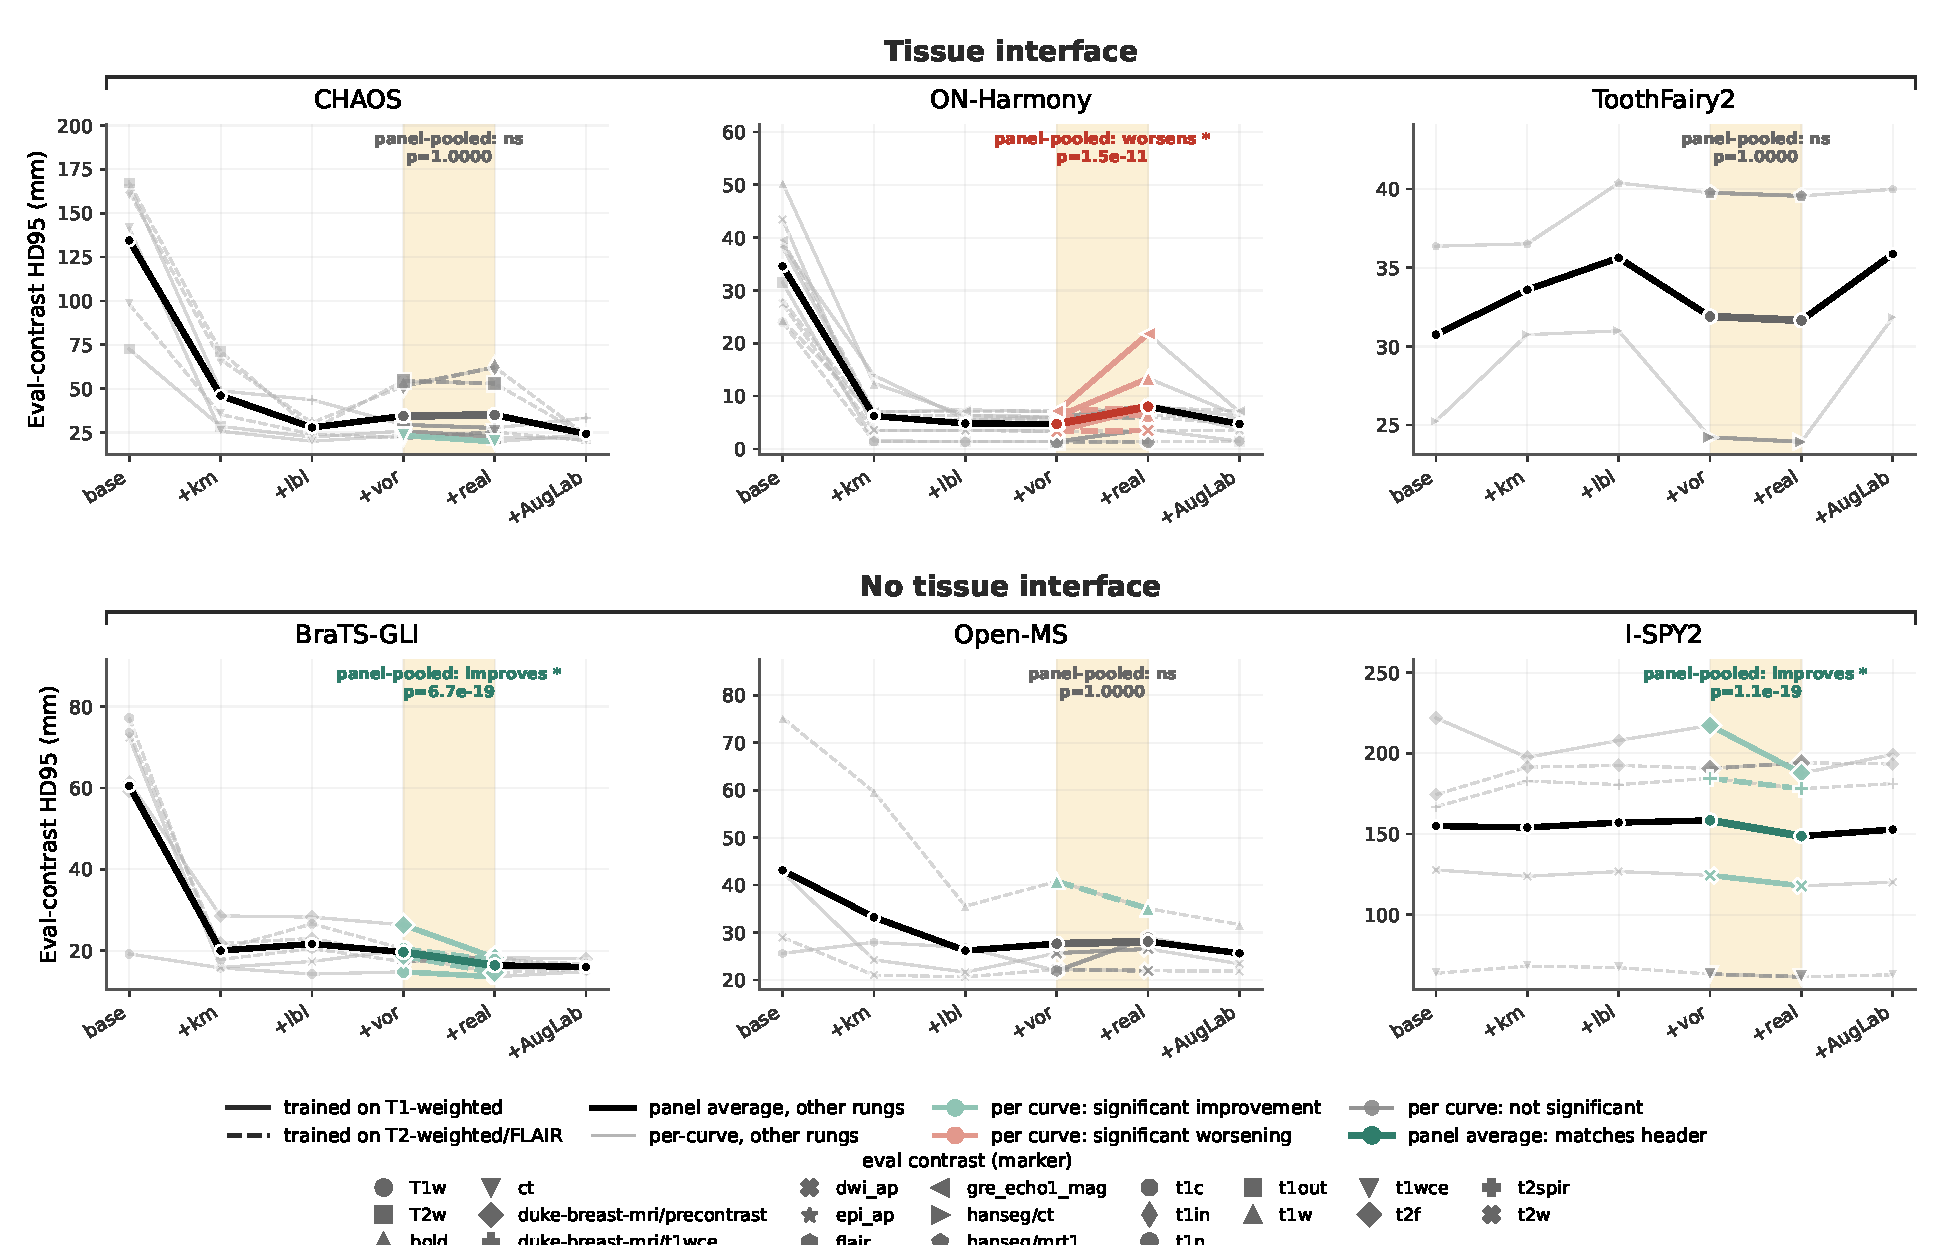
\includegraphics[width=\linewidth]{figures/per_contrast_curves/fill_swap_per_contrast_hd95}
\caption{The causal-ablation ladder of \cref{fig:ladder} (main paper), same
per-dataset panels, same boundary-type grouping, same fill-swap rung and
same visual scheme (per-curve colour only on the real-fill segment; bold
black panel average; one panel-pooled $p$-value per panel), reported on
HD95 instead of Dice (\emph{improvement} means the fill-swap step lowers
HD95, since lower is better here). The separation is messier than Dice:
only two of four panels reach panel-pooled significance -- BraTS-GLI
improves, ON-Harmony worsens -- while CHAOS and Open-MS are
not significant, so HD95 disagrees with Dice most in exactly the two
tasks (CHAOS, Open-MS) where the pooled effect is otherwise weakest.
Underlying deltas in \cref{tab:dissociation-hd95}.}
\label{fig:ladder-hd95}
\end{figure*}

\begin{table}[t]
\centering
\small
\setlength{\tabcolsep}{4pt}
\begin{tabular}{llc}
\toprule
Task & boundary type & $\Delta$ HD95 (mm) \\
\midrule
CHAOS T1in      & tissue interface   & $-2.95$ \\
CHAOS T2spir    & tissue interface   & $+4.20$ \\
ON-Harmony T1w  & tissue interface$^\dagger$ & $+6.22$ \\
ON-Harmony T2w  & tissue interface$^\dagger$ & $+0.38$ \\
ToothFairy2 CBCT & tissue interface$^\ddagger$ & $-0.25$ \\
\midrule
Open-MS FLAIR   & no tissue interface & $-3.02$ \\
Open-MS T1w     & no tissue interface & $+3.94$ \\
Brats-GLI T1n   & no tissue interface & $-4.59$ \\
Brats-GLI T2w   & no tissue interface & $-1.88$ \\
I-SPY2 T1-CE    & no tissue interface & $-18.09$ \\
I-SPY2 T2w      & no tissue interface & $-1.55$ \\
\bottomrule
\end{tabular}
\caption{Same fill-swap step as \cref{tab:dissociation} (main paper),
reported on HD95 instead of Dice (negative is better), all six tasks, both
training modalities each where two exist. The separation is not clean on
HD95 anywhere: the sign flips between the two modalities of the same task
for both Open-MS and CHAOS, so we restrict the dissociation claim to Dice in
the main paper and report HD95 here rather than presenting it as confirming
that claim. The two newest tasks do not rescue it either, for opposite
reasons: ToothFairy2 moves by a quarter of a millimetre ($p=0.59$), and
I-SPY2 T1-CE's $-18$mm is by far the largest movement in the table but comes
from a task whose absolute HD95 is $150$--$175$mm, where a single recovered
lesion focus shifts the $95$th percentile a long way.
$^\dagger$Grouped with CHAOS as tissue-interface, not a separate category
-- see \S4.3 of the main paper. $^\ddagger$Cross-dataset held-out axis
(HaN-Seg), as in \cref{tab:dissociation}.}
\label{tab:dissociation-hd95}
\end{table}

\paragraph{Full ladder: numbers and significance.} \cref{fig:ladder} (main
paper) shows the rung sequence visually; \cref{tab:ladder-full} gives the
underlying OOD Dice at every rung, with significance for each step against
the rung immediately before it (Holm-corrected paired Wilcoxon test within
each ladder's transitions). Most steps that add an ingredient help,
significantly, as expected. Eight cells are significant \emph{decreases}
(marked $\downarrow$), and they fall into three groups. The fill-swap step
on both ON-Harmony modalities (T1w and T2w), consistent with ON-Harmony's
tissue-interface grouping (\cref{subsec:e-ablation}) and replicating across
modalities. The Voronoi sub-parcellation step on Brats-GLI T1n (not T2w),
and the $k$-means and label-remap steps on the Breast ladders, where the
early partition-only rungs cost accuracy before the real-intensity fill
recovers it and more.

The third group is the one that explains \S\ref{subsec:e-main}: the final
$+$AugLab rung is a significant \emph{decrease} on Mandible ($69.2
\rightarrow 65.6$) and on Breast T2w ($35.8 \rightarrow 32.9$) --- the two
tasks where the complete method does not win. On both, PALETTE alone (the
$+$real rung) is at the ladder's maximum and the surrounding Auglab recipe
takes it back down. That localises the shortfall to the wrapper rather than
to the transform this paper argues for, and it is visible here in the same
per-rung numbers that carry the positive results, not in a separate analysis
constructed after the fact. We have not diagnosed which Auglab operator is
responsible; that is a question for the pipeline it belongs to.

We likewise do not hide that Voronoi's own marginal contribution is
task-dependent rather than uniformly positive -- a separate paired
significance check (same protocol as \cref{tab:mechanism}'s all-contrast
Dice, not just the OOD slice used above) confirms the same pattern: Voronoi
significantly \emph{helps} Open-MS FLAIR and (by a small margin) ON-Harmony
T1w, is flat on CHAOS T1in, and significantly \emph{hurts} Brats-GLI T1n
under the real-fill deployed configuration as well, not only here under
noise fill. The full method still wins on Brats-GLI T1n regardless
(\cref{tab:meta}): whatever Voronoi costs there is more than recovered by
the subsequent real-intensity fill step, so the net effect of the complete
pipeline is positive even though one internal component is not.

\begin{table}[t]
\centering
\scriptsize
\setlength{\tabcolsep}{2.4pt}
\resizebox{\linewidth}{!}{%
\begin{tabular}{lcccccccc}
\toprule
Rung & Open-MS & Open-MS & Brats-GLI & Brats-GLI & CHAOS & CHAOS & ON-Harm. & ON-Harm. \\
     & FLAIR   & T1w     & T1n       & T2w       & T1in  & T2spir & T1w     & T2w \\
\midrule
base       & 2.5 & 1.1 & 16.9 & 6.0 & 21.0 & 21.2 & 15.0 & 25.6 \\
+km        & $11.2^{**}$ & $9.8^{***}$ & $38.4^{***}$ & $38.6^{***}$ & $84.2^{***}$ & $79.0^{***}$ & $62.5^{***}$ & $63.5^{***}$ \\
+lbl       & $17.5^{***}$ & $22.4^{***}$ & $41.8^{***}$ & $40.2^{***}$ & $87.7^{***}$ & $83.4^{***}$ & 62.9 & 63.6 \\
+vor       & $19.6^{*}$ & $34.1^{***}$ & $39.8^{***}{\downarrow}$ & 41.0 & 87.2 & 82.7 & $63.2^{*}$ & $64.2^{***}$ \\
+real      & $27.3^{***}$ & 34.9 & $47.0^{***}$ & 41.5 & $88.2^{***}$ & 81.6 & $58.7^{***}{\downarrow}$ & $62.7^{***}{\downarrow}$ \\
+AL(v000)  & 30.6 & 36.4 & 46.9 & $46.8^{***}$ & 87.6 & 86.3 & $64.2^{*}$ & 63.9 \\
+AL(v100)  & 31.3 & 34.7 & $47.6^{*}$ & $46.9^{*}$ & 87.1 & $87.1^{*}$ & 64.2 & 64.4 \\
\bottomrule
\end{tabular}%
}

\vspace{0.6em}
\resizebox{\linewidth}{!}{%
\begin{tabular}{lccc}
\toprule
Rung & Mandible & Breast & Breast \\
     & CBCT     & T1-CE  & T2w \\
\midrule
base       & 39.9 & 13.9 & 32.6 \\
+km        & $64.7^{***}$ & $22.0^{***}$ & $31.4^{***}{\downarrow}$ \\
+lbl       & $65.9^{***}$ & $20.5^{***}{\downarrow}$ & $29.9^{***}{\downarrow}$ \\
+vor       & $68.6^{***}$ & 20.3 & $32.2^{***}$ \\
+real      & 69.2 & $24.0^{***}$ & $35.8^{***}$ \\
+AL(v000)  & $65.6^{***}{\downarrow}$ & $28.0^{***}$ & $32.9^{***}{\downarrow}$ \\
+AL(v100)  & $65.7^{**}$ & --- & --- \\
\bottomrule
\end{tabular}%
}
\caption{OOD Dice (\%) at every ladder rung (\cref{fig:ladder}, main paper),
all six tasks, both training modalities each where two exist, with
significance for each step vs.\ the rung immediately above it:
$^{*}p<0.05$, $^{**}p<0.01$, $^{***}p<0.001$ (Holm-corrected paired
Wilcoxon, within-ladder family of tests), $\downarrow$ marks a significant
\emph{decrease}. Rungs: base(line), +$k$-means, +label-remap, +Voronoi
(noise fill), +real-intensity fill (PALETTE alone), +AugLab (val000/val100).
The two newest tasks (lower block) have no val100 arm: I-SPY2's was never
trained, and ToothFairy2's was trained but not evaluated on the
cross-dataset half that forms its OOD axis, so no comparable figure exists.
Mandible's OOD axis is cross-dataset (HaN-Seg), as elsewhere.}
\label{tab:ladder-full}
\end{table}

\paragraph{Per-label breakdown: is the fill-swap effect uniform within a task?}
\label{par:per-label}
\cref{fig:ladder} shows that Brats-GLI T2w's pooled fill-swap effect is
small and not significant, with one significantly negative eval contrast
inside it (T2w$\to$T1n). This raises a further question: within that one
(training, eval) pair, does the fill-swap step affect every anatomical
sub-region equally, or is the worsening itself concentrated in specific
labels? We break Brats-GLI T2w$\to$T1n down by its four labels -- necrotic
core (NCR), oedema (SNFH), enhancing tumour (ET), resection cavity (RC);
$n=70$ test cases for SNFH and ET, present in essentially every case
(NCR $n=51$, RC $n=67$, since not every tumour has a necrotic core or a
resection cavity).

\begin{table}[h]
\centering
\small
\setlength{\tabcolsep}{4pt}
\begin{tabular}{lccc}
\toprule
Label & T1n$\to$T2w & T2w$\to$T1n & gap \\
\midrule
NCR  & 21.5 & 19.3 & $+2.1$ \\
SNFH & 66.3 & 45.3 & $\mathbf{+21.0}$ \\
ET   & 27.5 & 27.9 & $-0.4$ \\
RC   & 52.3 & 43.1 & $+9.1$ \\
\bottomrule
\end{tabular}
\caption{Absolute OOD Dice (\%) of the deployed real-fill (v26\_6\_2) model,
per label, both transfer directions.}
\label{tab:per-label-abs}
\end{table}

\begin{table}[h]
\centering
\small
\setlength{\tabcolsep}{4pt}
\begin{tabular}{lcc}
\toprule
Label & T1n$\to$T2w $\Delta$ & T2w$\to$T1n $\Delta$ \\
\midrule
NCR  & $+1.9$ (p=0.10) & $+0.3$ (p=0.87) \\
SNFH & $\mathbf{+14.7}$ (p=4.3e-11) & $\mathbf{-9.8}$ (p=4.5e-05) \\
ET   & $+2.3$ (p=0.017) & $+0.9$ (p=0.38) \\
RC   & $+2.9$ (p=0.0003) & $\mathbf{-6.5}$ (p=0.0039) \\
\bottomrule
\end{tabular}
\caption{Fill-swap step (+voronoi noise fill $\to$ v26\_6\_2 real fill),
per label, both directions. $p$: Holm-corrected paired Wilcoxon, family =
the 4 labels within each direction. \textbf{Bold} = significant.}
\label{tab:per-label-delta}
\end{table}

The worsening is not a property of ``the tumour'' -- it is concentrated
almost entirely in SNFH, which alone accounts for $+21.0$ of the roughly
14-point whole-tumour Dice gap between directions, and is the only label
whose fill-swap delta significantly reverses sign between the two training
directions ($+14.7$ when trained on T1n, $-9.8$ when trained on T2w). RC
shows the same reversal at smaller magnitude. NCR shows no significant
effect in either direction, and ET helps a little only in the direction
that already works (T1n$\to$T2w), never significantly reversing when
trained on T2w. \cref{fig:snfh-et-zoom} shows why on one representative
case: the T2w-trained model's real-fill prediction on SNFH collapses to a
thin band near the ventricle relative to its own noise-fill prediction on
the same case, while its ET prediction looks essentially unchanged between
the two rungs.

\begin{figure}[h]
\centering
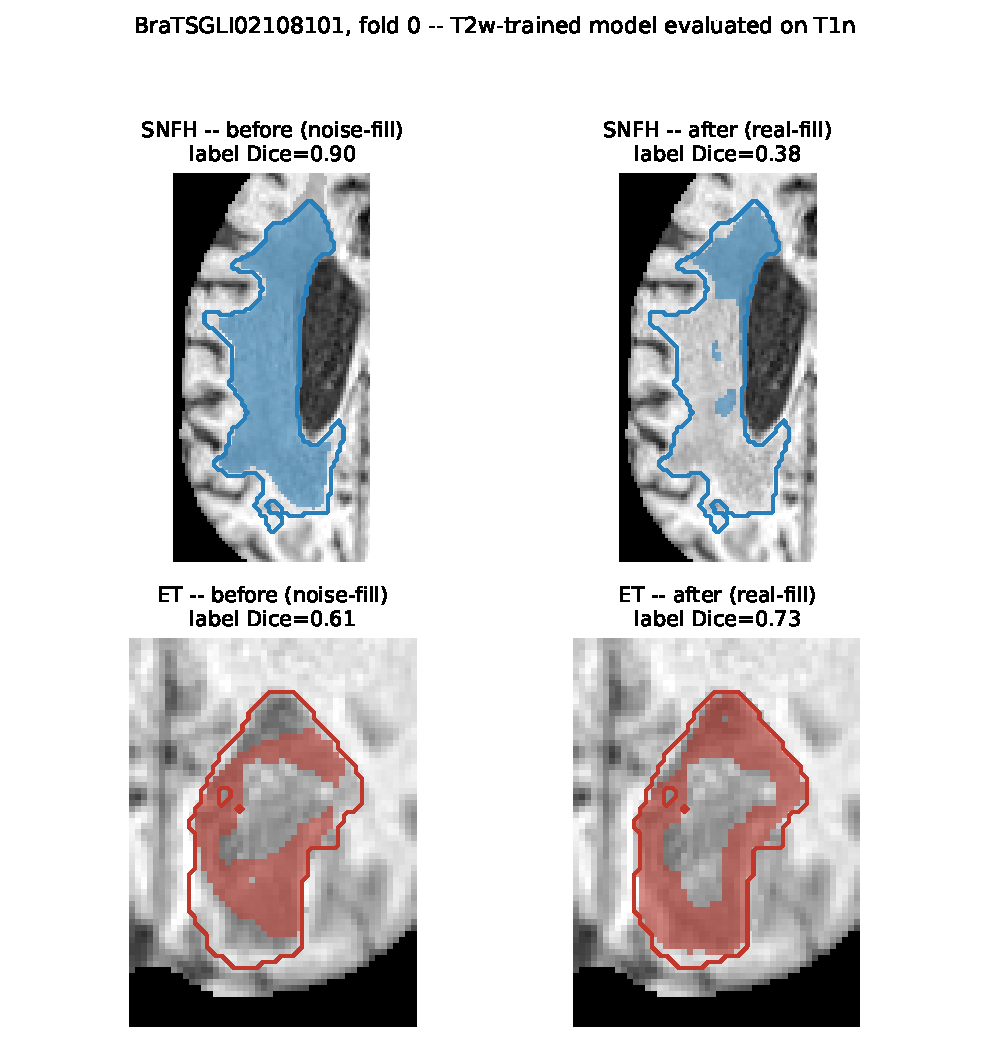
\includegraphics[width=0.85\linewidth]{figures/snfh_et_zoom}
\caption{\texttt{BraTSGLI02108101}, fold 0, T2w-trained model evaluated on
T1n. Zoomed crops before (noise-fill) and after (real-fill) the fill-swap
step, for the SNFH-dominant (top) and ET-dominant (bottom) lesion
components of the same case. Colour = ground truth wherever the prediction
agrees; grey = false positive; outline = ground truth.}
\label{fig:snfh-et-zoom}
\end{figure}

One candidate mechanism, flagged for future work rather than tested here:
a texture pattern learned from one contrast's rendering of a diffuse,
texture-defined label like oedema may not simply fail to transfer to a
different contrast's rendering of the same tissue -- it may actively
mislead, if the model has come to rely on a contrast-specific cue that the
other contrast does not reproduce. This would be an instance of shortcut
learning~\cite{geirhos2020shortcut} -- specifically, a network relying on a
domain-specific cue that does not reproduce across acquisition protocols,
the mechanism~\citet{ouyang2023causality} identify behind failed
single-source domain generalization in cross-modality and cross-sequence
medical segmentation -- rather than the intended, causal feature, which a
simplicity-biased network need not prefer even when it would generalize
better~\cite{shah2020simplicity}. We have not tested this mechanistically
here; it is the most concrete hypothesis consistent with the label-specific,
direction-dependent pattern above, not a demonstrated cause.

\section{Synthetic contrast at validation time}
\label{sec:suppl-val100}

Throughout the main paper PALETTE is applied with synthetic contrast during
training only (\emph{train050/val000}), because every competing method is
likewise evaluated with a real-contrast validation set; this keeps the
comparison exactly like-for-like. PALETTE can additionally be applied to the
validation set, so that model selection is performed under randomized
contrast as well (\emph{train050/val100}).

\begin{table}[t]
\centering
\small
\setlength{\tabcolsep}{4pt}
\begin{tabular}{lcc|cc}
\toprule
 & \multicolumn{2}{c|}{Dice $\uparrow$} & \multicolumn{2}{c}{HD95 (mm) $\downarrow$} \\
Task & val000 & val100 & val000 & val100 \\
\midrule
Brats-GLI    & 46.8 & \textbf{47.3} & 15.2 & \textbf{14.7} \\
CHAOS        & 85.0 & \textbf{85.2} & 30.6 & \textbf{28.7} \\
ON-Harmony   & 68.2 & \textbf{68.4} &  4.2 & \textbf{4.1}  \\
Open-MS      & \textbf{38.5} & 37.9 & 24.3 & \textbf{24.2} \\
\midrule
\textbf{mean (4 tasks)} & 59.6 & \textbf{59.7} & 18.6 & \textbf{17.9} \\
\bottomrule
\end{tabular}
\caption{Applying PALETTE at validation time as well as at training time.
Restricted to the four tasks where both configurations exist: Mandible's
val100 arm was trained but never evaluated on the cross-dataset half that
forms its OOD axis, and Breast's was never trained, so neither can appear
here. The mean row is therefore over those four tasks in both columns --- it
is a within-configuration comparison on a fixed task set, not the cross-task
average the main paper declines to report. The two configurations are
statistically indistinguishable
at task level (Dice $p = 0.49$, HD95 $p = 0.93$, same task-stratified test
as \cref{tab:meta}), so we report the like-for-like \emph{val000}
configuration in the main paper and note \emph{val100} as a free additional
gain where it helps -- it requires no extra data, annotation or training
cost, only applying the same transform to the validation split. Open-MS's
own Dice moves the other way (38.5 $\to$ 37.9), which keeps \textbf{overall}
Dice an effective wash across the two configurations (59.6 vs.\ 59.7, not a
significant difference) despite three of the four tasks favoring val100.}
\label{tab:suppl-val100}
\end{table}

Validation-time randomization improves most tasks on both metrics
(\cref{tab:suppl-val100}), most visibly on boundary distance for CHAOS
($30.6 \rightarrow 28.7$~mm). The effect is not significant at task level,
and Open-MS Dice moves slightly the other way, so we do
not claim it as a separate contribution; we report it because it costs
nothing and because it indicates that the benefit of contrast randomization
extends to model selection and is not confined to the gradient updates.

\section{Component ablation}
\label{sec:suppl-mechanism}

\label{subsec:e-mechanism}
% moved from the main text 2026-08-02 to fit the 8-page limit

To attribute the gain of the full method to its individual components,
rather than to synthetic-contrast augmentation in general, we build an
additive ablation ladder on top of the no-augmentation anchor (\emph{Base},
\cref{subsec:e-main}): first the unsupervised $k$-means intensity partition
alone (\S\ref{subsec:m-transform}, step~1); then the anatomical label-remap
step (step~4); then the Voronoi spatial sub-parcellation (step~2); and
finally the full signed affine remap of \cref{eq:affine} (step~3), which
together constitute PALETTE in its entirety and is denoted \textbf{Ours} in
this ladder --- identical to the standalone (no-Auglab) configuration used
throughout \cref{subsec:e-main}. Every rung is evaluated without Auglab, so
that the ladder isolates PALETTE's own internal components from the
separate question of whether it composes with a prior augmentation
pipeline, which we address next. The synthetic-data fraction is fixed at
$50\%$ of training iterations throughout, as one of several augmentation
constants (alongside, e.g., the $k$-means class count and the affine
magnitude range of \S\ref{subsec:m-transform}) that are set once and not
tuned per dataset; validation uses real-contrast data only (no synthetic
contrast at validation time).

\begin{table}[t]
\centering
\small
\setlength{\tabcolsep}{4pt}
\begin{tabular}{lcccc}
\toprule
Component & CHAOS & Open-MS & BraTS & ON-Harmony \\
\midrule
Base (no augmentation)                & 36.1 & 25.2 & 25.3 & 27.5 \\
\quad + $k$-means partition           & 84.8 & 30.6 & 40.6 & 67.6 \\
\quad + label remap                   & 87.7 & 34.6 & 43.2 & 68.0 \\
\quad + Voronoi sub-parcellation      & 87.2 & 36.1 & 41.8 & 68.2 \\
\quad + affine remap (\textbf{Ours})  & 87.9 & 40.4 & 47.4 & 63.6 \\
\midrule
\quad + Auglab (deployed)             & 87.4 & 39.5 & 46.4 & 68.6 \\
\bottomrule
\end{tabular}
\caption{Mechanism ablation (top five rows, additive, no Auglab) and
deployment composability check (bottom row). Each rung adds exactly one
PALETTE component on top of the row above; all-modality Dice (\%),
averaged over held-out test contrasts, folds 0--2, train fraction $50\%$.
BraTS and ON-Harmony report their T1n/T1w settings, matching every other
table in this paper. The deployed row matches \cref{tab:suppl-dice}'s
\textbf{Ours} column exactly.}
\label{tab:mechanism}
\end{table}

\paragraph{Composability with Auglab.} PALETTE is deployed, throughout this
paper, as one additional operator inside the Auglab pipeline rather than as
a replacement for it (\cref{subsec:e-setup}); Auglab is a full prior
augmentation method in its own right, not a component of PALETTE, so
stacking it on top of the ladder above is a composability/deployment check,
not a further mechanism-ablation step. \cref{tab:mechanism} keeps the two
separate: the top five rows isolate PALETTE's internal mechanism, evaluated
with no Auglab throughout, while the bottom row reports PALETTE plus Auglab
--- the configuration used everywhere else in this paper --- set apart by a
rule rather than presented as the next rung of the same ladder.



\section{Direct measurement of texture fidelity}
\label{sec:suppl-ngf}

\begin{figure}[t]
\centering
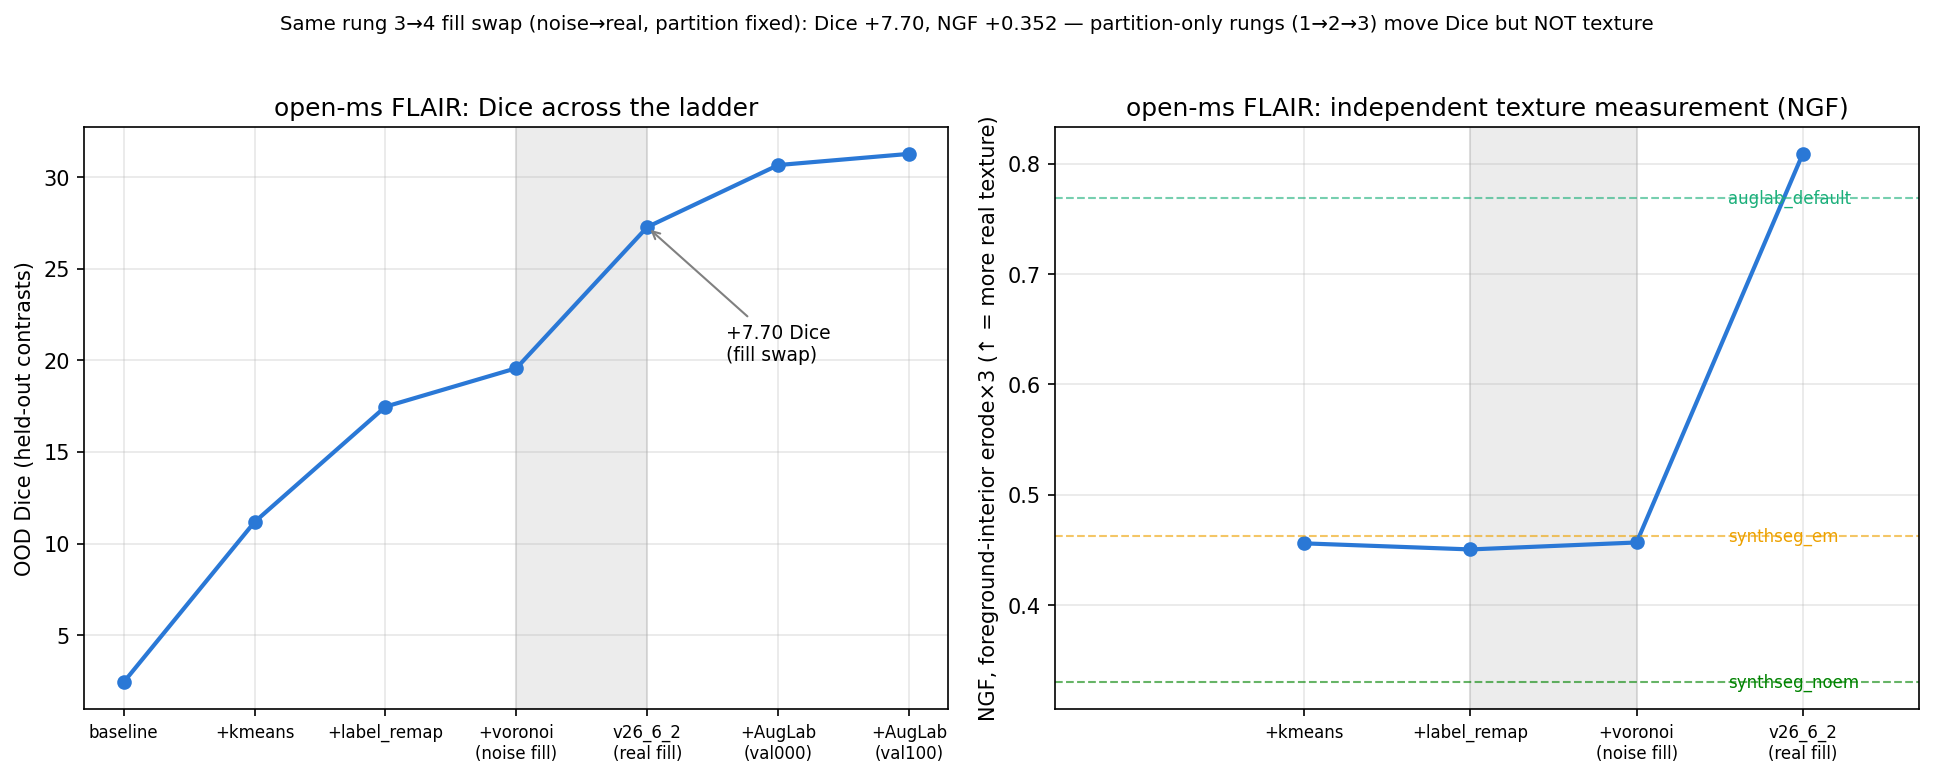
\includegraphics[width=\linewidth]{figures/ngf_dose_response_openms_flair}
\caption{Downstream Dice (left) against an independent, segmentation-free
measurement of texture fidelity (right, NGF gradient-orientation agreement
with the source volume) across the rung sequence. The three noise-fill rungs
sit flat at the texture floor while their Dice still rises -- those gains come
from richer contrast randomization, not texture. Both quantities jump together
at the fill swap, which is the step the texture hypothesis predicts.}
\label{fig:ngf-dose}
\end{figure}

The Dice ablation above
The ablation of \cref{subsec:e-ablation} shows that texture preservation
\emph{matters} downstream; here we measure the texture itself, directly and
without reference to any segmentation.
For each method we compute the normalized-gradient-field (NGF)
similarity~\cite{haber2006ngf} between the augmented image and the source
scan --- an alignment-of-gradients measure that is high when local edge and
texture structure is retained and near the isotropic-noise floor
($\approx\!1/3$) when it is destroyed. \cref{tab:ngf} reports mean NGF over
$n{=}30$ scans on the two Open-MS contrasts. PALETTE retains far more of the
source texture than any noise-based method and significantly more than
Auglab (FLAIR $p=7.6\times10^{-3}$, T1w $p=1.2\times10^{-6}$), while the
label-style methods (SynthSeg-EM, noise-fill) and especially SynthSeg-noEM
sit near the noise floor --- exactly the ordering the mechanism predicts, and
consistent with the downstream Dice gaps of \cref{tab:dissociation}.

\begin{table}[t]
\centering
\small
\setlength{\tabcolsep}{6pt}
\begin{tabular}{lcc}
\toprule
Method & FLAIR & T1w \\
\midrule
\textbf{PALETTE} & \textbf{0.808} & \textbf{0.894} \\
Auglab           & 0.772 & 0.777 \\
SynthSeg-EM      & 0.461 & 0.422 \\
noise-fill       & 0.453 & 0.401 \\
SynthSeg-noEM    & 0.332 & 0.319 \\
\bottomrule
\end{tabular}
\caption{Texture fidelity measured by NGF similarity to the source scan
(mean over $n{=}30$ Open-MS scans; higher = more source texture retained,
$\approx\!1/3$ = isotropic-noise floor). PALETTE preserves the most texture;
the noise-based methods sit near the floor.}
\label{tab:ngf}
\end{table}

